\documentclass[a4paper, 10pt]{article}
\usepackage[utf8]{inputenc}
\usepackage{verbatim}
\usepackage{listings}
\usepackage{graphicx}
\usepackage{a4wide}
\usepackage{color}
\usepackage{amsmath}
\usepackage{amssymb}
\usepackage[dvips]{epsfig}
\usepackage[toc,page]{appendix}
\usepackage[T1]{fontenc}
\usepackage{cite} % [2,3,4] --> [2--4]
\usepackage{shadow}
\usepackage{hyperref}
\usepackage{titling}
\usepackage{marvosym }
\usepackage{subcaption}
\usepackage[noabbrev]{cleveref}

\renewcommand{\topfraction}{.85}
\renewcommand{\bottomfraction}{.7}
\renewcommand{\textfraction}{.15}
\renewcommand{\floatpagefraction}{.66}
\renewcommand{\dbltopfraction}{.66}
\renewcommand{\dblfloatpagefraction}{.66}
\setcounter{topnumber}{9}
\setcounter{bottomnumber}{9}
\setcounter{totalnumber}{20}
\setcounter{dbltopnumber}{9}


\setlength{\droptitle}{-10em}   % This is your set screw

\setcounter{tocdepth}{2}

\lstset{language=c++}
\lstset{alsolanguage=[90]Fortran}
\lstset{basicstyle=\small}
\lstset{backgroundcolor=\color{white}}
\lstset{frame=single}
\lstset{stringstyle=\ttfamily}
\lstset{keywordstyle=\color{red}\bfseries}
\lstset{commentstyle=\itshape\color{blue}}
\lstset{showspaces=false}
\lstset{showstringspaces=false}
\lstset{showtabs=false}
\lstset{breaklines}
\title{FYS3150 - Project 5\\
Financial Modelling}
\author{Daniel Heinesen, Gunnar Lange}
\begin{document}
\maketitle
\begin{abstract}
We investigate a range of different models for the behavior of financial agents interacting with each other, aiming to extract an equilibrium distribution. We begin with a straightforwards Monte Carlo model, where two financial agents randomly split their wealth among each other. We expand this model by including the possibility of agents saving money, and by modifying the probability of an interaction by taking into account financial proximity and the effect of previous transactions. This is further developed by introducing some analytic solutions, to which we compare our simulations, and by an investigation into the way in which we can assert whether or not equilibrium has been reached.
\end{abstract}
\tableofcontents
\section{Introduction}
Monte Carlo simulations of financial agents is at the core of the relatively new, interdisciplinary, field of econophysics. There has been a veritable landslide of such models presented in recent papers \textbf{INSERT REFERENCES HERE}, ranging from simple models, where all agents have the same interaction probability and simply redistribute their money, to far more complex models including savings, financial proximity or psychological propinquity.\\
\linebreak
We present an overview of four models with varying degrees of complexity, in which we try to extract and understand the equilibrium distributions, as well as some some indicators of equilibrium. We begin with a theoretical overview of our four models, presenting the models, as well as some analytic solutions which exist for some of the models. We continue with a brief overview of our methods, including both how we implement the models and how we assess the equilibration point in our model. We then present our results and a discussion thereof.
\section{Theoretical model}
In this section we introduce the theoretical model necessary to model financial agents through Monte Carlo simulations. We also introduce the analytic solutions, wherever they are exist. 
\subsection{Simulating financial transactions}
We begin all our simulations with $N$ agents, each with a certain amount of wealth $m_i$, where $i \in [1, N]$.  For simplicity, we let all our agents begin with an equal amount of initial wealth, $m_i=m_j$ for $i,j \in [1,N]$. We subsequently let all agents interact with each other, according to four different set of rules, presented below. We let this interaction continue until equilibrium has been achieved, and we repeat these simulations until we have a sufficient amount of statistical data. The details of how this is done can be found in section \ref{Method_section}.
\subsubsection{Initial model for the interaction between two financial agents (model A)}\label{Initial_model}
We begin with a simple model for the interaction of two financial agents, which was initially devised \textbf{HERE}. Assume that we, at random, pick two agents $i$ and $j$, each with wealth given by $m_i$ and $m_j$. We model the interaction between $m_i$ and $m_j$ as a complete, unbiased, exchange of wealth, that is; the agents combine their wealth, and then redistribute it by drawing a random number, $\epsilon$ $\in [0,1]$, from a uniform distribution, and then redistributing the wealth according to:
\begin{equation}
m_1'=\epsilon(m_1+m_2)
\end{equation}
\begin{equation}
m_2'=(1-\epsilon)(m_1+m_2)
\end{equation}
Where the primed quantities represent the wealth of each agent. Notice that the total wealth is conserved in this interaction, seeing as:
$$m_1'+m_2'=\epsilon(m_1+m_2)+(1-\epsilon)(m_1+m_2)=m_1+m_2$$
Thus we are only redistributing wealth among our agents.
\subsubsection{First modification: Implementing savings (model B)}\label{Model_B}
We expand our model slightly by including the possibility of our agents retaining a certain amount of money in the transaction, as thought up by \textbf{HERE}. This is modelled by a parameter $\beta$, which describes the fraction of money saved by each agent. With this modification, we can rewrite the equations describing our interaction as:
\begin{equation}
\begin{split}
m_i'=\lambda m_i+\epsilon(1-\lambda)(m_i+m_j) \\
m_j'=\lambda m_j+(1-\epsilon)(1-\lambda)(m_i+m_j)
\end{split}
\end{equation}
Note that the total amount of wealth is still conserved, seeing as:
$$m_i'+m_j'=\lambda m_i+\epsilon(1-\lambda)(m_i+m_j)+\lambda m_j+(1-\epsilon)(1-\lambda)(m_i+m_j)=\lambda (m_i+m_j)+(1-\lambda)(m_i+m_j)=m_i+m_j$$
Thus we are still only redistributing wealth, but according to a different probability distribution. Note further that model A and model B are identical if $\lambda = 0$.
\subsubsection{Second modification: Including the effect of proximity (model C)}\label{Model_C}
Our second modification is inspired by an idea published \textbf{HERE}. Here, we introduce the possibility of two chosen agents not interacting at all, that is; we introduce a probability of interaction. We construct this probability in a biased way; making it more likely for agents with comparable amount of wealth to interact with each other. Specifically, we determine the probability of an interaction occurring between agents $i$ and $j$, $p_{ij}$, from the equation:
\begin{equation}\label{eq:Nearest_neighbors}
p_{ij}=|m_i-m_j|^{-\alpha} 
\end{equation}
Where $\alpha$ is a positive parameter which we vary. Thus whenever we have drawn two agents $i$ and $j,$ from our population, we also compute $p_{ij}$, and compare it to a random number, $\epsilon \in [0,1]$, drawn from a uniform distribution. If $\epsilon < p_{ij}$, the transaction occurs, otherwise, no transactions take place. We will implement this model both with and without savings (with $\lambda > 0$ and with $\lambda=0$), and attempt to extract the behavior for different $\alpha$.
\subsubsection{Final modification: Including the previous transactions (model D)}\label{Model_D}
Our final modification is based on an article published \textbf{HERE}. We include an "acquaintance factor", or a psychological propinquity, where the likelihood of a transaction occurring scales with the number of previous transactions between two agents $i$ and $j$. This is a simple modification of equation \ref{eq:Nearest_neighbors}, which we implement as:
\begin{equation}\label{eq:nearest_with_previous_transactions}
p_{ij}=|m_i-m_j|^{-\alpha}(c_{ij}+1)^{\gamma}
\end{equation} 
Where $c_{ij}$ is the number of previous interactions between agents $i$ and $j$ and $\gamma$ is a positive parameter which we vary. The additional $1$ is added to make it possible for agents that have not previously interacted to perform a transaction. Note that this model is initially identical to the model in equation \ref{eq:Nearest_neighbors}, but deviates at later times.
\subsection{Analytic solutions}\label{Analytic_solution}
In this section we present analytic solutions, wherever they are available. Model A and model B have analytic solutions, found \textbf{HERE} which we can use to test the consistency of our simulations directly. We also know approximately how we expect the tail of our other distributions (the richest agents) to behave.
\subsubsection{Analytic solution to the initial model (model A)}
The model from section \ref{Initial_model}, has an analytic solution which is described in detail \textbf{HERE}. There, it is shown that the equilibrium distribution, in the continuous limit, approaches a Gibbs distribution, of the form:
\begin{equation}\label{eq:Analytic_solution_A}
A(m)=\mu \exp(-\mu m)
\end{equation}
Where $\mu$ is a parameter which we have to determine. Note that, because $m$ (the amount of wealth) cannot be negative, this distribution is normalized\footnote{Because $\int_0^{\infty} \mu \exp(-\mu m)dm=1$}.
\subsubsection{Analytic solution to the first modification (model B)}
The model from section \ref{Model_B} also has an analytic solution in the continuous limit. This is described in detail \textbf{HERE}, where it is shown that the probability distribution, $B(m)$, approaches:
\begin{equation}
B(m)=\frac{n^n}{\Gamma(n)}m^{n-1}e^{-nm}
\end{equation}
Where $n$ is given by:
$$n=1+\frac{3\lambda}{1-\lambda}$$
Note that this enables us to determine $\mu$ from equation \ref{eq:Analytic_solution_A} directly; as noted in section \ref{Model_B}, model A and model B are identical for $\lambda = 0$. Thus, we expect \textbf{FINISH THIS, ASK DANIEL}.
\subsubsection{Analytic solution for the second and final modification (model C and D)}
For these models, we do not have analytic solutions readily available. However, as stated \textbf{HERE}, it is known from empirical studies that the richest agents in society (the high-end tail of our distribution) tend to follow a Pareto distribution, given by:
\begin{equation}\label{eq:Anayltic_solution_C_D}
C(m) \propto m^{-1-\beta}
\end{equation}
Where $\beta \in [1,2]$. Thus, we check how realistic our models are, by fitting a function of the form given in equation \ref{eq:Anayltic_solution_C_D} to the tail of our distribution, to see whether or not the richest agents follow the empirical Pareto distribution.
\section{Methods}\label{Method_section}
Here, we introduce the methods that we employ to ensure that we get sufficient, reliable, statistical data, as well as some technicalities relating to our numeric implementation of the models discussed in the previous section.
\subsection{Obtaining reliable data}
We only want to analyze steady-state distributions, where the final distribution stays approximately constant. Note that, due to the dynamic nature of our system, the distribution at any specific instance may vary quite substantially, even at equilibrium. Thus, extracting a single distribution after a given number of transactions will give rise to significant statistical uncertainty. Therefore, we perform many repetitions of each experiment, starting with the same initial configuration, and then average the distributions that we extract. We will refer to each such repetitions, consisting of a give number of transactions, as a Monte Carlo cycle.\\
\linebreak
Whether or not we get reliable results will therefore hinge on two criteria:
\begin{itemize}
\item Having a sufficient number of transactions per Monte Carlo cycle
\item Having a sufficient number of Monte Carlo cycles
\end{itemize}
We need to have enough transactions per Monte Carlo cycle for the system to "forget" its initial state - that is, we need to have enough transactions to ensure that we have achieved equilibrium in the system. As discussed above, however, the distribution from a single cycle, even at equilibrium, is prone to statistical fluctuations. Thus, to get reliable data, we will have to perform sufficient Monte Carlo cycles for the distribution to stabilizes.\\
\subsubsection{Ensuring we perform a sufficient number of transactions}
A simple, yet efficient, way to investigate the number of transactions that we require, is to write out the variance of our distribution as a function of the number of transactions for a single Monte Carlo cycle. We compute the variance of the distribution as:
\begin{equation}
\mathrm{Var}(x)=\frac{\langle m^2 \rangle - \langle m \rangle^2 }{n}
\end{equation}
Where $\langle m \rangle$ denotes the mean of the distribution of wealth (which in our case is always the initial amount of wealth, as we start with a uniform distribution) and $n$ is the number of performed transactions.\\
\linebreak
Because we start with a uniform distribution of wealth, the variance will start out at zero. We expect it to subsequently increase with more transactions and finally to stabilizes, fluctuating around some value. We determine the number of transactions to be the point where the variance stabilizes.
\subsubsection{Determining the number of Monte Carlo cycles needed}
We determine the number of Monte Carlo cycles needed by looking at the difference in the average of the distribution between two subsequent Monte Carlo cycles. We calculate this difference as:
\begin{equation}\label{eq:Relative_diff_MC_steps}
\delta = |\vec{M}_{i}-\vec{M}_{i-1}|
\end{equation}
Where $\vec{M}$ is a vector with $N$ components, containing the wealth of each agent. $M_i$ represents the \textit{average wealth} after $i$ Monte Carlo cycles (i.e. the average of the distributions from all previous Monte Carlo cycles), and $M_{i+1}$ represents the same average, but with an additional Monte Carlo cycle taken into account. We expect $\delta$ to approach zero as the number of Monte Carlo cycles increases, as the statistical fluctuations from each cycles cancel each other out for a sufficiently large number of cycles. Notice, however, that additional Monte Carlo cycles incur additional computation time, which quickly racks up. Therefore, we choose a number of Monte Carlo cycles which balances computational feasibility with a low enough $\delta$. 
\subsection{Implementing the Monte Carlo simulations}
As the main algorithm for simulating the transactions is relatively short, we present, in Pseudo-Code, the program for computing model A below:
\lstinputlisting{Pseudo_code_simple_walkers.cpp}
Note that the other models can be easily implemented by expanding the loop over transactions slightly.
\subsection{Determining the number of bins}
\section{Results and discussion}
\subsection{Results from the initial model (model A)}
\subsubsection{Results from our investigation into the optimal combination of parameters}
The results from our investigation into the optimal parameters for our initial model are shown below:
\begin{figure}[!ht]
    \centering
    \begin{subfigure}[H!]{0.5\textwidth}
        \centering
        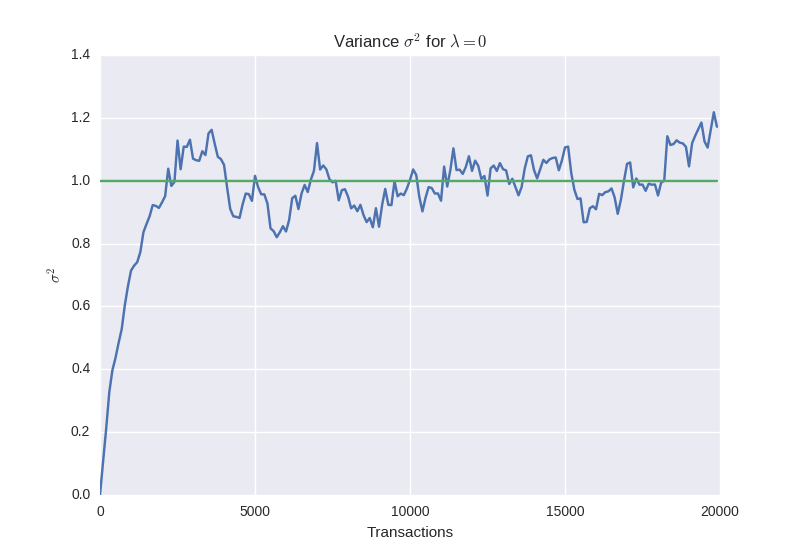
\includegraphics[height=2.0in]{varLamb0.png}
        \caption{The variance of a single Monte Carlo cycle}\label{fig:ModelA_Var}
    \end{subfigure}%
    ~ 
    \begin{subfigure}[H!]{0.5\textwidth}
        \centering
        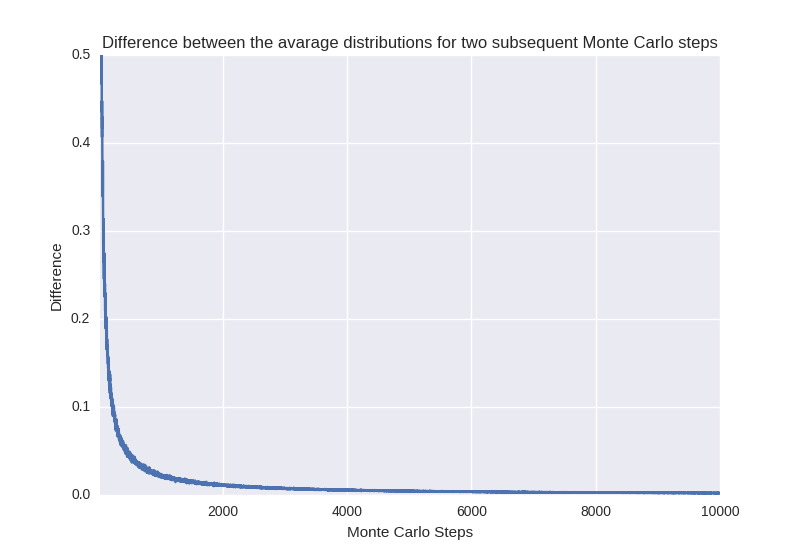
\includegraphics[height=2.0in]{diffMCLamb0.png}
        \caption{The difference in the distribution for successive Monte Carlo steps}\label{fig:ModelA_MC_steps}
    \end{subfigure}
    \caption{Plots from our investigation into the optimal choice of parameters. Figure \ref{fig:ModelA_Var} shows how the variance of our distribution evolves with the number of transactions. This is for a single Monte Carlo cycle, with $N=500$ agents, and the initial wealth, $m0=500$. In figure \ref{fig:ModelA_MC_steps}, we show how the difference between successive average distributions evolves with the number of Monte Carlo steps. Each Monte Carlo step consists of $N=500$ agents, which interact with a total of $10^4$ transactions. Note that the $x$-axis does not start at zero, for a better graphical presentation of the long-term development.}\label{fig:ModelA}
\end{figure} %ASK DANIEL ABOUT m0
\subsubsection{The distribution from model A}

We discuss later how we decide on a combination of parameters. We present the final, average, distribution, for this combination of parameters, below:
\begin{figure}[!ht]
\centering
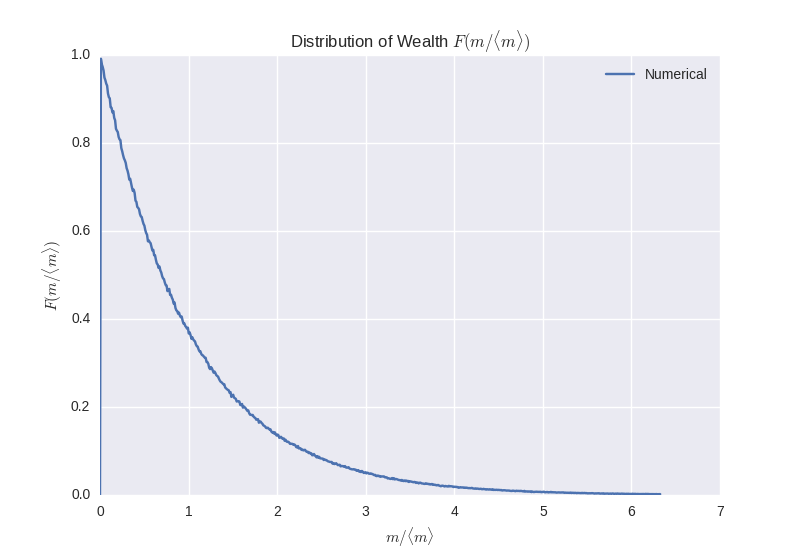
\includegraphics[height=2.5in]{distLamb0.png}
\caption{The final distribution of wealth from model A. Here $\langle m \rangle$ is the average wealth, which equals the initial wealth per agent, $m_0=500$. This simulation was run with $500$ agents, performing $10^4$ transactions per Monte Carlo cycles, with a total of $10^4$ Monte Carlo cycles.}\label{fig:ModelA_final_distribution}
\end{figure}
\subsubsection{Comparison with the analytic model}
We also include a logarithmic plot, of the above distribution, together with the analytic solution from section \ref{Analytic_solution}, to investigate how well our numerical distribution fits our analytic model.
\begin{figure}[!ht]
    \centering
    \begin{subfigure}[H!]{0.5\textwidth}
        \centering
        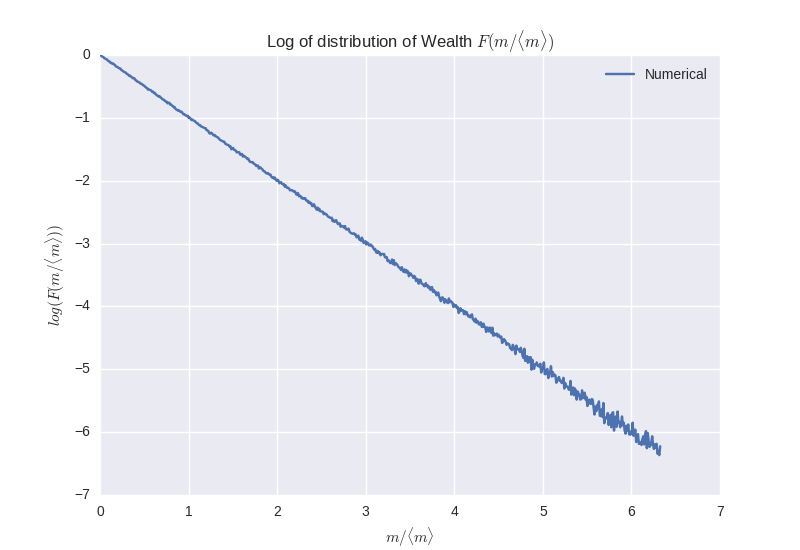
\includegraphics[height=2.0in]{logDistLamb0.png}
        \caption{A logarithmic plot of figure \ref{fig:ModelA}}\label{fig:ModelA_log_raw}
    \end{subfigure}%
    ~ 
    \begin{subfigure}[H!]{0.5\textwidth}
        \centering
        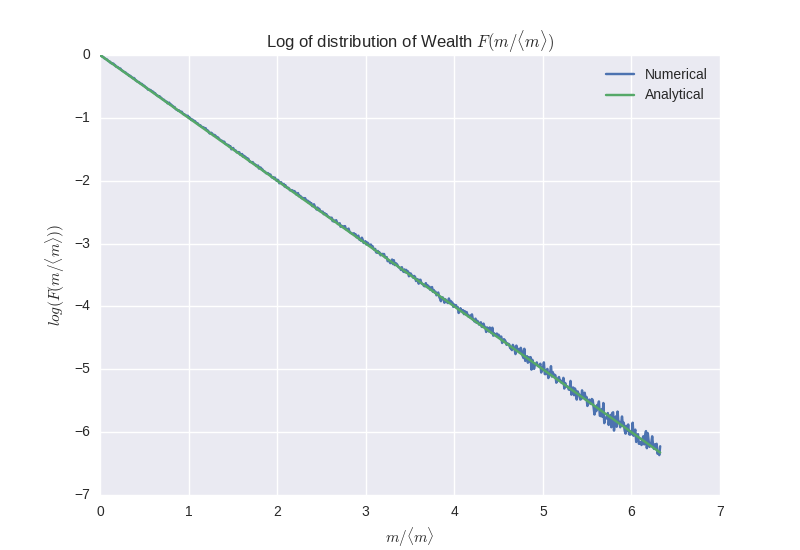
\includegraphics[height=2.0in]{logDistLamb0WAnalyt.png}
        \caption{The same plot, with a linear fit.}\label{fig:ModelA_log_fit}
    \end{subfigure}
    \caption{A logarithmic plot of figure \ref{fig:ModelA}, used to determine the analytic expression for the distribution in figure \ref{fig:ModelA}}\label{fig:ModelA__log}
\end{figure}
Finally, we include the distribution from Model A, together with the analytic plot, to determine how well our analytic model fits our results.
\begin{figure}[!ht]
\centering
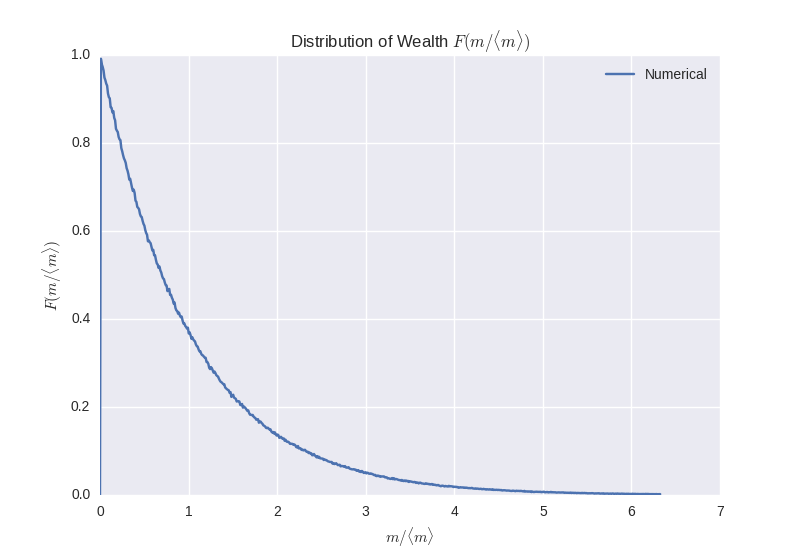
\includegraphics[height=2.5in]{distLamb0.png} %FIX THIS
\caption{Plot of figure \ref{fig:ModelA_final_distribution} together with the analytic solution from section \ref{Analytic_solution}}\label{fig:ModelA_final_distribution_with_analytic}
\end{figure}
\subsection{Discussion of model A}
\subsubsection{Choosing parameters}
As seen in figure \ref{fig:ModelA_Var}, the variance from a single run stabilizes after a few thousand interactions for this model. Note that this will, in general, depend upon the number of agents, as we need to ensure that every agent performs approximately the same number of transactions to get good statistical data. In our case, we have 500 agents. We therefore choose to perform $10^4$ Monte Carlo cycles, as we can see that the variance has stabilized at this point. This gives an average of 40 transactions per agent (as every transaction involves two agents), which should ensure that every agent is involved in at least a few transactions.\\
\linebreak
Figure \ref{fig:ModelA_MC_steps} shows the difference in the distribution between two successive Monte Carlo steps, as described by equation \ref{eq:Relative_diff_MC_steps}. For the first few cycles, this difference is very large (a difference of up to 35), but it quickly falls. We can see that the difference between two successive cycles quickly approaches zero. We choose $10^4$ Monte Carlo cycles as our cutoff point, where the difference is small enough to be essentially zero, but our simulations still run very quickly.
\subsubsection{The distribution}
As can be seen in figure \ref{fig:ModelA_final_distribution_with_analytic}, the analytic model agrees excellently with our simulations. The only exception is the very beginning: far fewer people have almost no wealth than predicted by the analytic model. This is not particularly surprising, however. The amount of wealth given to each agent at each transaction in this model depends on the number $\epsilon$, which is a floating point number in the interval $[0,1]$. Note, however, that the probability of $\epsilon$ being either exactly zero or exactly 1 is infinitesimal,  %ASK: EXACTLY ZERO?
(as these are floating point numbers). For an agent to end up with no wealth after a transaction, $\epsilon$ has to be one of these extreme values. Therefore, there are no agents with zero wealth. %LOOK AT THIS AGAIN


\subsection{Results from the first modification (model B)}
\subsubsection{Results from our investigation into the optimal combination of parameters}
The results from our investigation into the optimal parameters for model B, for various values of the saving factor $\lambda$,  are shown below:
\begin{figure}[!ht] %Fix this figure
    \centering
    \begin{subfigure}[H!]{0.5\textwidth}
        \centering
        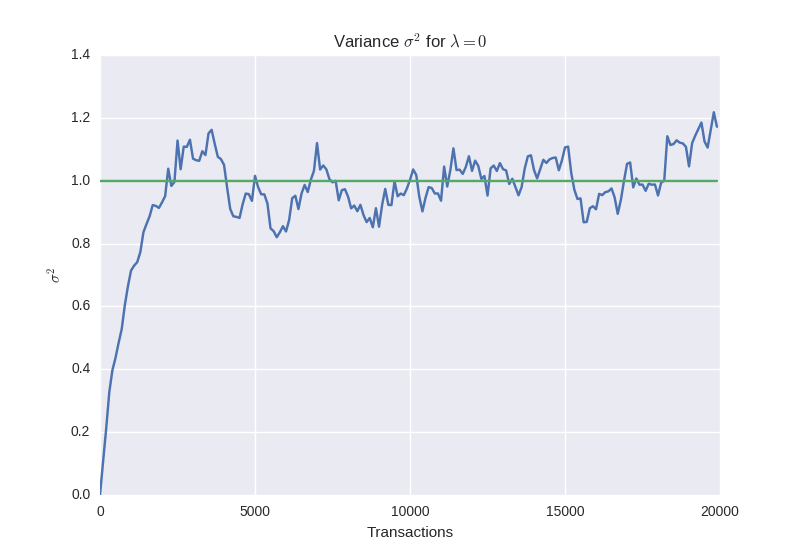
\includegraphics[height=2.0in]{varLamb0.png}
        \caption{The variance of a single Monte Carlo cycle in model B}\label{fig:ModelB_Var}
    \end{subfigure}%
    ~ 
    \begin{subfigure}[H!]{0.5\textwidth}
        \centering
        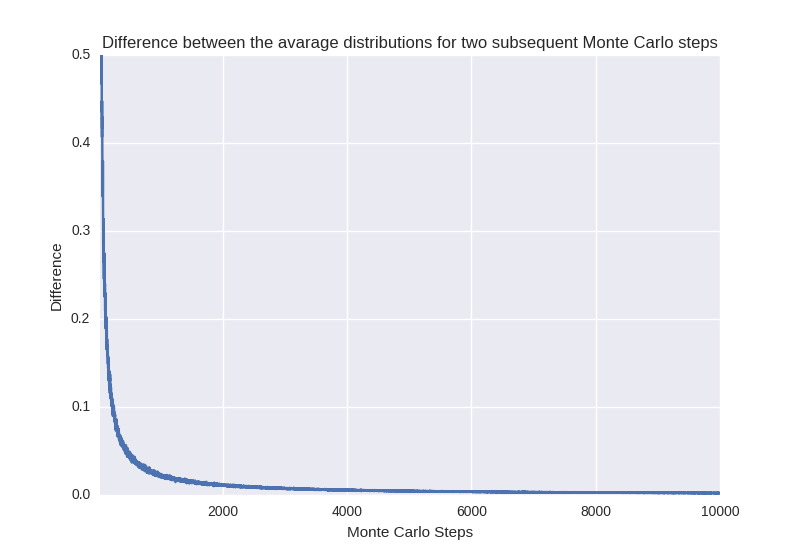
\includegraphics[height=2.0in]{diffMCLamb0.png}
        \caption{The difference in the distribution for successive Monte Carlo steps in model B}\label{fig:ModelB_MC_steps}
    \end{subfigure}
    \caption{Plots from our investigation into the optimal choice of parameters. Figure \ref{fig:ModelB_Var} shows how the variance the distribution for model B evolves with the number of transactions. This is for a single Monte Carlo cycle, with $N=500$ agents, and the initial wealth, $m0=500$. In figure \ref{fig:ModelB_MC_steps}, we show how the difference between successive average distributions evolves with the number of Monte Carlo steps. Each Monte Carlo step consists of $N=500$ agents, which interact with a total of $10^4$ transactions. Note that the $x$-axis does not start at zero, for a better graphical presentation of the long-term development.}\label{fig:ModelB}
\end{figure} %ASK DANIEL ABOUT m0
\subsubsection{The distribution from model B}
We postpone a discussion of the choice of parameters until the discussion part later. We present the final, average, distribution, for this combination of parameters, below:
\begin{figure}[!ht]
\centering
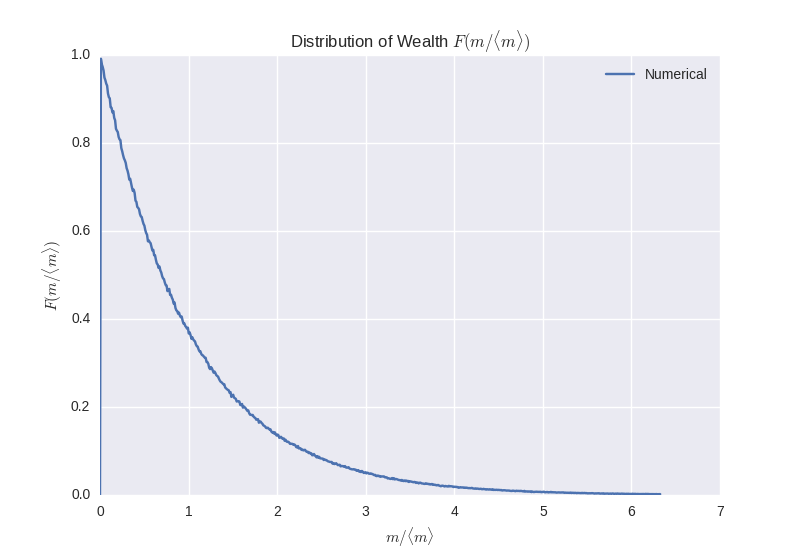
\includegraphics[height=2.5in]{distLamb0.png} %Fix this one
\caption{The final distribution of wealth from model B. Here $\langle m \rangle$ is the average wealth, which equals the initial wealth per agent, $m_0=500$. This simulation was run with $500$ agents, performing $10^4$ transactions per Monte Carlo cycles, with a total of $10^4$ Monte Carlo cycles.}\label{fig:ModelB_final_distribution}
\end{figure}
\subsubsection{Comparison with the analytic model}
We also include a plot, of the above distribution, together with the analytic solution from section \ref{Analytic_solution}, to investigate how well our numerical distribution fits our analytic model.
\begin{figure}[!ht]
\centering
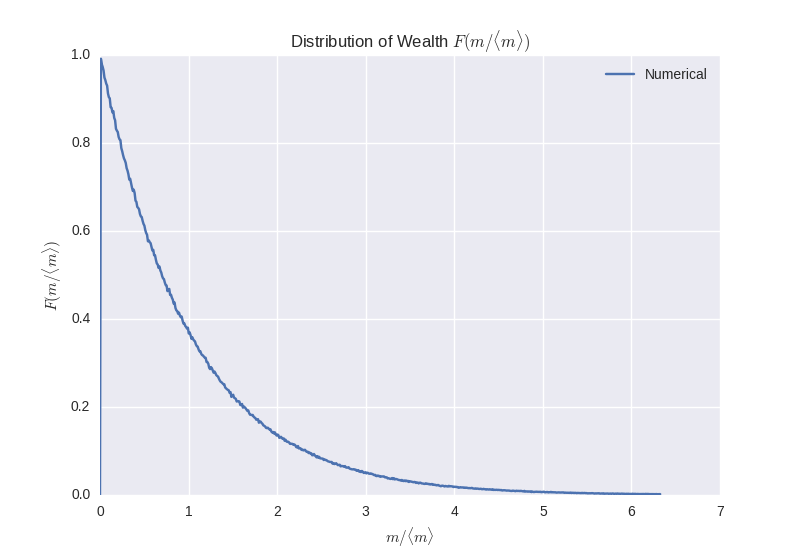
\includegraphics[height=2.5in]{distLamb0.png} %Fix this one
\caption{Figure \ref{fig:ModelB_final_distribution}, together with the analytic solution from section \ref{Analytic_solution}.}\label{fig:ModelB_final_distribution_with_analytic}
\end{figure}
\subsection{Discussion of model B}
\subsubsection{Choosing parameters}

\subsubsection{The distribution}

\subsection{Results from the second modification (model C)}
\subsubsection{Results from our investigation into the optimal combination of parameters}
The results from our investigation into the optimal parameters for model C, for various combinations of the saving factor $\lambda$ and the closeness factor $\alpha$ are shown below:
\begin{figure}[!ht] %Fix this figure
    \centering
    \begin{subfigure}[H!]{0.5\textwidth}
        \centering
        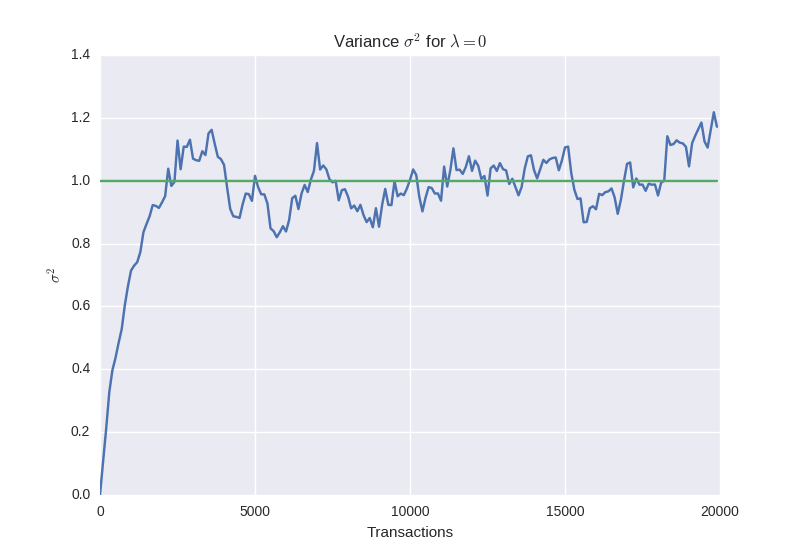
\includegraphics[height=2.0in]{varLamb0.png}
        \caption{The variance of a single Monte Carlo cycle in model C}\label{fig:ModelC_Var}
    \end{subfigure}%
    ~ 
    \begin{subfigure}[H!]{0.5\textwidth}
        \centering
        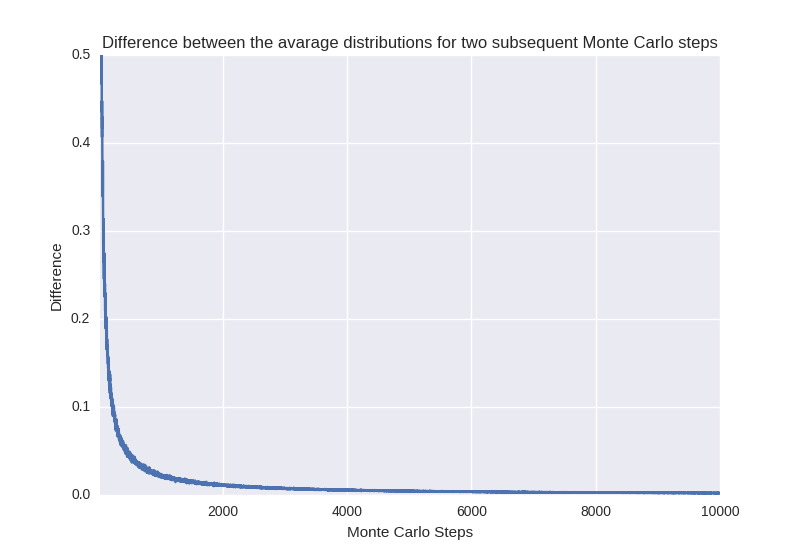
\includegraphics[height=2.0in]{diffMCLamb0.png}
        \caption{The difference in the distribution for successive Monte Carlo steps in model C}\label{fig:ModelC_MC_steps}
    \end{subfigure}
    \caption{Plots from our investigation into the optimal choice of parameters. Figure \ref{fig:ModelB_Var} shows how the variance the distribution for model B evolves with the number of transactions. This is for a single Monte Carlo cycle, with $N=500$ agents, and the initial wealth, $m0=500$. In figure \ref{fig:ModelB_MC_steps}, we show how the difference between successive average distributions evolves with the number of Monte Carlo steps. Each Monte Carlo step consists of $N=500$ agents, which interact with a total of $10^4$ transactions. Note that the $x$-axis does not start at zero, for a better graphical presentation of the long-term development.}\label{fig:ModelC}
\end{figure} %ASK DANIEL ABOUT m0
\subsubsection{The distribution from model C}
We again postpone a discussion of the choice of parameters until the discussion part later. We present the final, average, distribution, for this combination of parameters, below:
\begin{figure}[!ht]
\centering
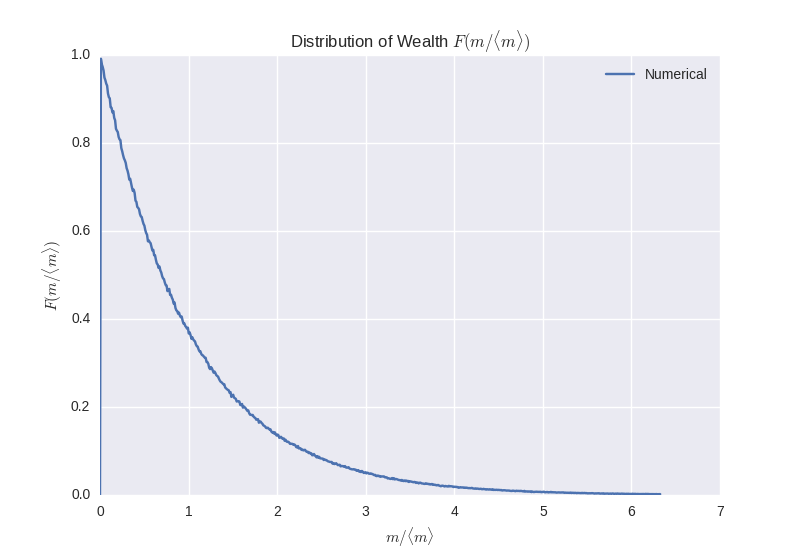
\includegraphics[height=2.5in]{distLamb0.png} %Fix this one
\caption{The final distribution of wealth from model C. Here $\langle m \rangle$ is the average wealth, which equals the initial wealth per agent, $m_0=500$. This simulation was run with $500$ agents, performing $10^4$ transactions per Monte Carlo cycles, with a total of $10^4$ Monte Carlo cycles.}\label{fig:ModelC_final_distribution}
\end{figure}
\subsubsection{Comparison with the analytic model}
As stated in section \ref{Analytic_solution}, we do not have an analytic expression for the entire distribution. However: if our model accurately depicts reality, then the higher end of the distribution should approximately follow a Pareto distribution. We show a fit of the form given in equation \ref{eq:Anayltic_solution_C_D}, applied to the tail of the distribution, in the figure below.
\begin{figure}[!ht]
\centering
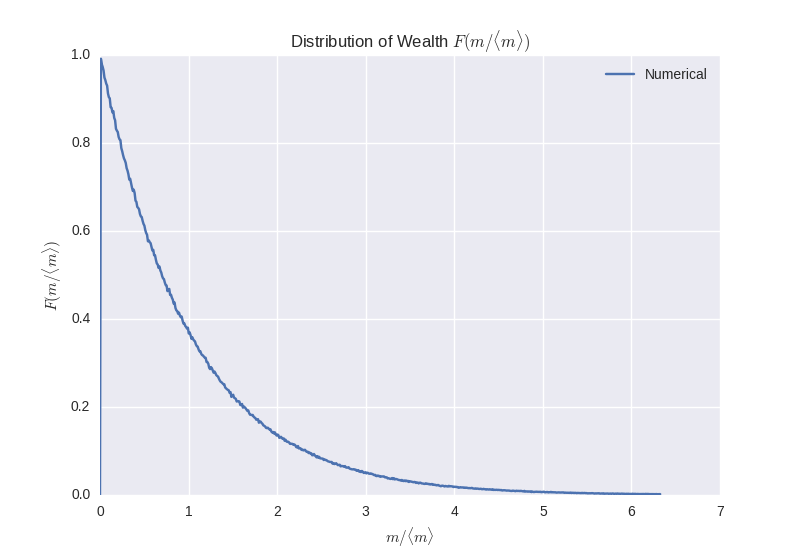
\includegraphics[height=2.5in]{distLamb0.png} %Fix this one
\caption{Figure \ref{fig:ModelC_final_distribution}, together with the analytic solution from section \ref{Analytic_solution}.}\label{fig:ModelC_final_distribution_with_analytic}
\end{figure}
\subsection{Discussion of model C}
\subsubsection{Choosing parameters}

\subsubsection{The distribution}

\subsection{Results from the final modification (model D)}
\subsubsection{Results from our investigation into the optimal combination of parameters}
The results from our investigation into the optimal parameters for model D, for various values of the saving factor $\lambda$, the interaction factor $\lambda$ and the psychological propinquity factor $\gamma$  are shown below:
\begin{figure}[!ht] %Fix this figure
    \centering
    \begin{subfigure}[H!]{0.5\textwidth}
        \centering
        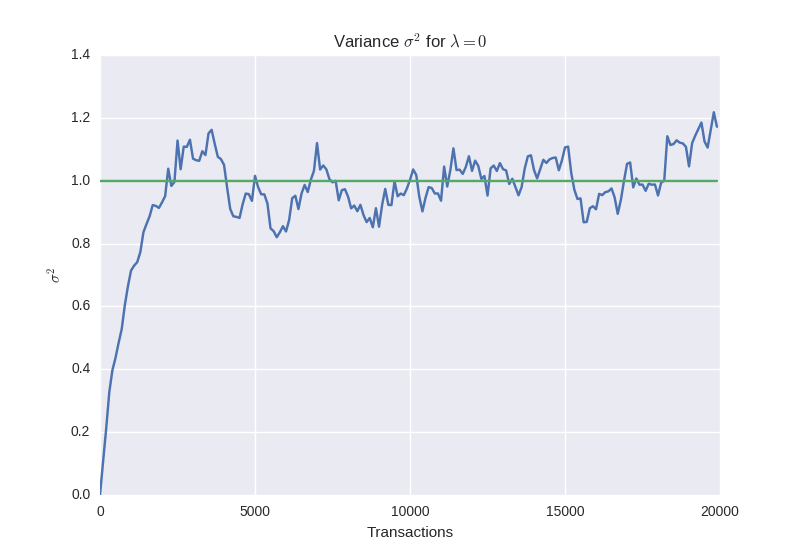
\includegraphics[height=2.0in]{varLamb0.png}
        \caption{The variance of a single Monte Carlo cycle in model D}\label{fig:ModelD_Var}
    \end{subfigure}%
    ~ 
    \begin{subfigure}[H!]{0.5\textwidth}
        \centering
        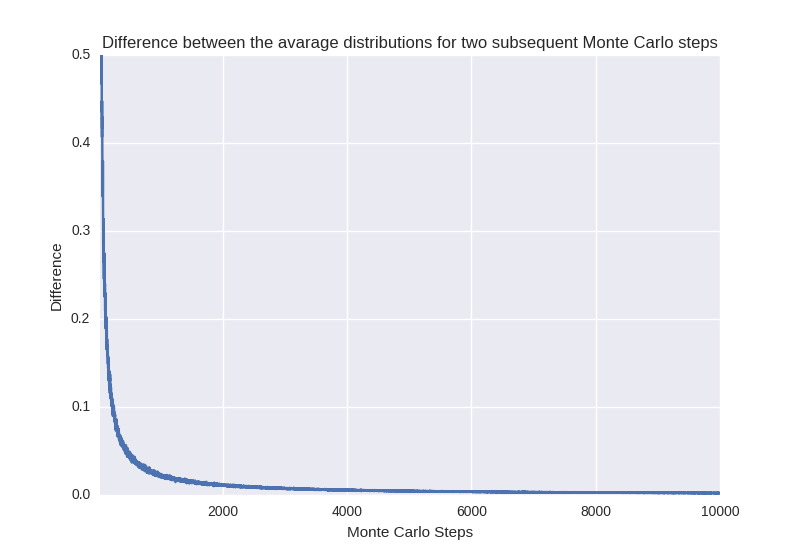
\includegraphics[height=2.0in]{diffMCLamb0.png}
        \caption{The difference in the distribution for successive Monte Carlo steps in model B}\label{fig:ModelD_MC_steps}
    \end{subfigure}
    \caption{Plots from our investigation into the optimal choice of parameters. Figure \ref{fig:ModelD_Var} shows how the variance the distribution for model B evolves with the number of transactions. This is for a single Monte Carlo cycle, with $N=500$ agents, and the initial wealth, $m0=500$. In figure \ref{fig:ModelB_MC_steps}, we show how the difference between successive average distributions evolves with the number of Monte Carlo steps. Each Monte Carlo step consists of $N=500$ agents, which interact with a total of $10^4$ transactions. Note that the $x$-axis does not start at zero, for a better graphical presentation of the long-term development.}\label{fig:ModelD}
\end{figure} %ASK DANIEL ABOUT m0
\subsubsection{The distribution from model D}
We postpone a discussion of the choice of parameters until the discussion part later. We present the final, average, distribution, for this combination of parameters, below:
\begin{figure}[!ht]
\centering
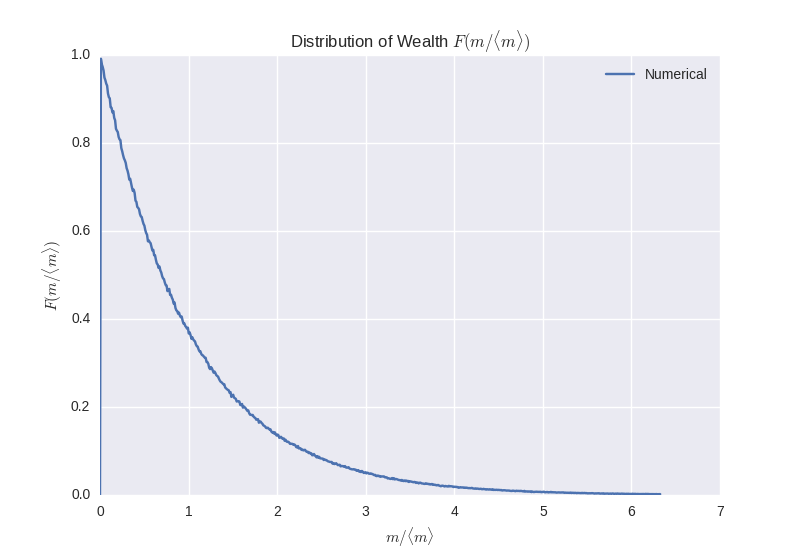
\includegraphics[height=2.5in]{distLamb0.png} %Fix this one
\caption{The final distribution of wealth from model B. Here $\langle m \rangle$ is the average wealth, which equals the initial wealth per agent, $m_0=500$. This simulation was run with $500$ agents, performing $10^4$ transactions per Monte Carlo cycles, with a total of $10^4$ Monte Carlo cycles.}\label{fig:ModelD_final_distribution}
\end{figure}
\subsubsection{Comparison with the analytic model}
We also include a plot, of the above distribution, together with the analytic solution from section \ref{Analytic_solution}, to investigate how well our numerical distribution fits our analytic model.
\begin{figure}[!ht]
\centering
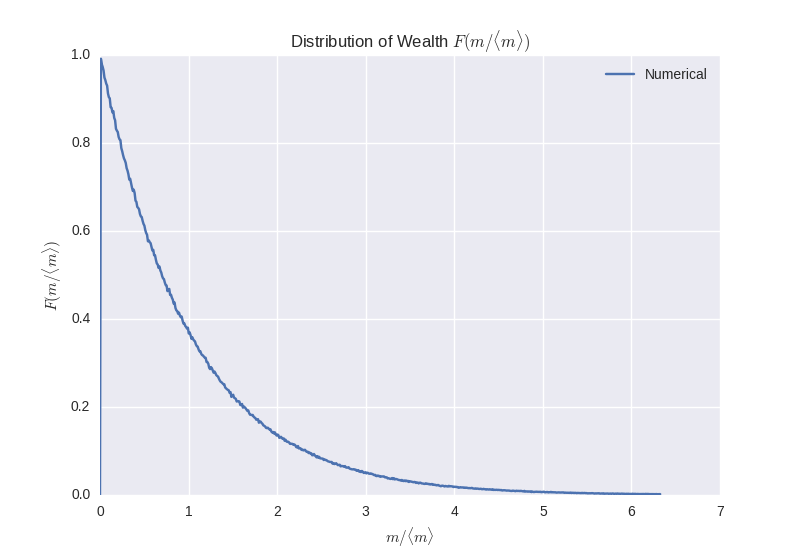
\includegraphics[height=2.5in]{distLamb0.png} %Fix this one
\caption{Figure \ref{fig:ModelB_final_distribution}, together with the analytic solution form section \ref{Analytic_solution}.}\label{fig:ModelD_final_distribution_with_analytic}
\end{figure}
\subsection{Discussion of model D}
\subsubsection{Choosing parameters}

\subsubsection{The distribution}



\section{Conclusion}
\subsection{Conclusion}
\subsection{Outlook}
\end{document}

%%INCLUDE INITIAL MONEY